\documentclass[12pt, a4paper]{book}
\begin{document}\label{chap:Method_ML}
We have now presented the dataset and theory, and are thus ready to start making our ML algorithms. The first part of this chapter will be a presentation of the dataset in more details, included all the events and the \textit{weights} variable.
We will also explore how we divide our dataset into a training and testing set. Afterwards we will discuss the crucial task of optimizing the architecture and hyperparameters of the ML models for obtaining high-performance classifiers. In this field, the challenge is often to 
distinguish between signal events from rare physics phenomena, and the much more common SM background processes. Since the signals events are extremely rare, the classifiers need to be highly optimized in order to effectively separate them from 
the background. In addition, the datasets have numerous features, which can lead to overfitting or poor generalization if not properly optimized. Another hardship is how to mitigate the phenomena of \textit{jagged arrays} and missing variables.\\
\\It is essential to carefully choose the model architecture and hyperparameters, as well as the dataset pre-processing techniques, in order to achieve the best possible performance in the search for the rare DM physics phenomena. This can involve optimizing 
parameters such as the learning rate and the regularization strength. Exclusively for the NNs we have the number of layers and the number of neurons per layer. Exclusively for the BDTs we have the number of trees and the tree depth. The second and third part of this chapter will be just about optimization for the NNs and BDTs respectively.

\clearpage
\section{The datasets}
The way we are making datasets in this project, to keep it as close to model independent as possible, will be of the following format
\begin{itemize}
   \item Make a dataset with all the SM backgrounds and one DM model.
   \item Make a dataset with all the SM backgrounds and all the DM models, divided into different signal regions and statistically combine the results of each signal region
\end{itemize}
The idea behind the first one is to start with a model dependent approach, where we train an ML algorithm to learn just one model at a time. The reason for taking this approach, is because it is still closer to being more model independent than normal ML HEP searches, as these usually train on the whole SM background dataset with just one 
signal model with fixed masses and parameters. While what we would be doing is combining all the different masses and parameters into one dataset for each model.\\
\\For the second one, if we created Signal Regions (SR) in kinematically orthogonal regions, then some models might be more important than other in each region. Meaning that the approach would teach the ML algorithm the signatures of the DM physics in the final state, rather than making an algorithm that is good at learning one individual model.
Furthermore, the plan is to combine the results of each respective region to get an overall view of all the signal regions studied.\\
\\In this project we will look at real data from the ATLAS detector from all running periods of Run II. This is from period 2015-2016, 2017 and 2018 each with an integrated luminosity of $36.4, 44.3$ and 58.5 $fb^{-1}$, respectively. 
In Table \ref{tab:dataset} we list the overall number of corresponding MC simulated events for each process, together with the expected events (i.e. scaled to the relevant cross-section and integrated luminosity), for all SM background and the as DM models considered. In addition to using the features in Table \ref{tab:variables}, we will also include the EventID, dataset ID (DSID), period, 
dilepton final state, label telling us whether an event is signal or background and the \textit{weight} of each event.
\begin{table}[!h]
   \centering
    \caption[Dataset used for ML]{Table showcasing the number of simulated events and expected events for every SM background channel and DM model that will be used in this thesis.}
    \footnotesize\begin{tabular}{l|r|r}\midrule\midrule
      Channel                                                                         & Simulated Events            & Expected events for 139 fb$^{-1}$ \\\midrule
      W                                                                               & 38,684                & 5,436        \\
      Drell Yan                                                                       & 47,201,697            & 2,198,258    \\
      TTbar                                                                           & 28,126,697            & 978,531      \\
      Single top                                                                      & 729,624               & 93,899       \\
      Diboson                                                                         & 10,983,689            & 116,654      \\\midrule
      Standard model total                                                            & 87,080,391            & 3,392,777    \\\midrule
      $Z'$ Dark Higgs Heavy Dark Sector                                               & 498,621               & 54.92\footnote{The expected number of events for any BSM model has prefixed assumptions about for example cross-section, decay width, etc. As we do not empirically know if any of these assumptions are correct, these are not set in stone.}         \\
      $Z'$ Dark Higgs Light Dark Sector                                               & 892,365               & 155.37         \\
      $Z'$ Light Vector Heavy Dark Sector                                             & 521,759               & 39.82         \\
      $Z'$ Light Vector Light Dark Sector                                             & 470,352               & 235.70         \\
      $Z'$ Effective Field Theory Heavy Dark Sector                                   & 715,409               & 0.0004           \\
      $Z'$ Effective Field Theory Light Dark Sector                                   & 640,963               & 0.0007          \\
      Supersymmetric direct slepton production                                        & 684,276               & 413,044.46        \\
      2HDM + a                                                                        & 3,371,806             & 65,211.31         \\\midrule\midrule
   \end{tabular}
   \label{tab:dataset}
\end{table}
\newpage\noindent From this dataset we can see one of the main challenges that will follow throughout the thesis, especially with the model dependent approach. This is the unbalance of the dataset, as an example lets look at the DH HDS model using the model dependent approach. Here we would train using all 87,080,391 simulated background events and 498,621 simulated signal events, as the numbers 
show, the majority of the dataset consists of background events, making the task of learning harder for any ML algorithm. This becomes even harder when applying the weights used for re-weighting simulated events to expected events at 139 fb$^{-1}$. What these weights used are is the subject of the next section.

\subsection{Weights}\label{sec:wgts}
The weights are crucial for most of what is to come further in this thesis. The weights only apply to MC simulations and can be interpreted as corrections to the simulations. The weights are defined as Eq. (\ref{eq:wgts})
\begin{equation}\label{eq:wgts}
   W = w_{mc}\times w_{pu}\times w_{xs}\times w_{lsf} \times w_{nlo,ew} \times w_{ttbar} \times w_{jet} \times w_{bjet} \times \frac{\text{lumi}_{period}}{\sum w_{mc, DSID}}
\end{equation}
This equation has a lot of information in it, so every part of this will be discussed. Starting from the MC weight, $w_{mc}$, which as stated in \cite{Pythia} gives the relative probability of an event within a sample, the pile-up weight $w_{pu}$, is a weight used to correct object reconstruction as it can be possible for multiple objects to cross on the 
identification process. \cite{Soyez:2018opl}\\ 
\\The cross-section weight $w_{xs}$, defined as $w_{xs} := xs \times w_{kf} \times g_{eff}$ where $xs$ is the cross-section of the process, $w_{kf}$ is the $k-$factor which tries to take into account the higher-order QCD corrections, 
for more details we refer the reader to the study done by Catani et al. \cite{Catani:2001cr}. $g_{eff}$ is the filter efficiency, which is the expected fraction of MC events that pass through the acceptance criteria.\\
\\The Lepton and trigger Scale Factor (LSF), $w_{lsf}$, which are applied in order to correct for differences in reconstruction in MC with respect to data, the Next to Leading Order (NLO) electroweak correction $w_{nlo,ew}$, which corrects for higher order EW diagrams, 
for more details we refer the reader to the paper by Denner et al. \cite{Denner:2022pwc}. \\
\\The $w_{ttbar}, w_{jet}$ and $w_{bjet}$, which are reconstruction corrections for $t\overline{t}$ \cite{Czakon:2015owf}, jets \cite{ATLAS:2014hvo} and b-jets \cite{ATLAS:2019bwq}, respectively. And lastly the luminosity of the period, meaning
$$
\text{lumi}_{period} = \begin{cases}
               36.4\text{ fb}^{-1},& \text{for period = 2015-2016}\\
               44.3\text{ fb}^{-1},& \text{for  period = 2017}\\
               58.5\text{ fb}^{-1},& \text{for  period = 2018}
               \end{cases}
$$
divided by the Sum Of Weights (SOW), $\sum w_{mc}$ of every sample for each dataset ID.

\subsection{Signal regions}\label{sec:SRs}
As a first step towards achieving less model dependence we will create three Signal Regions (SR). The goal is then to train one network in each respective SR that contains all the DM models we wish to study. The SR we will study are defined below 
\begin{itemize}
   \item SR1: $m_{ll} >110$ GeV and $E_T^{miss} \in [50, 100]$ GeV
   \item SR2: $m_{ll} >110$ GeV and $E_T^{miss} \in [100, 150]$ GeV
   \item SR3: $m_{ll} >110$ GeV and $E_T^{miss} >150$ GeV
\end{itemize}
where the $m_{ll}$ cut is made such that we remove the $Z-$peak before training and where the MET regions are orthogonal. 
The goal of having kinematically orthogonal SRs when training is to allow the combination of the results.



\subsection{Train and test split}\label{sec:train_test}
When training our networks we will use 80\% of the dataset, the remaining 20\% will be used to test whether the networks are learning any physical patterns or just getting really good at guessing events in the given dataset. When splitting the datasets however, we need to be absolutely certain that the distributions 
follow the same shape and have the same ratio of background channels as well as having good MC and data agreement in the training and testing data sets. In this thesis we will utilize a function from \verb|scikit learn| \cite{scikit-learn} called \verb|train_test_split| which can easily split our dataset into 
a training and testing set of a chosen size, while also splitting the label of the dataset, meaning whether the event is signal or background, in the same manner.
\graphicspath{{../../../Plots/Data_Analysis/train_test_split/}}
\begin{figure}[!ht]
	\centering
	\begin{subfigure}[b]{0.49\textwidth}
        \centering
        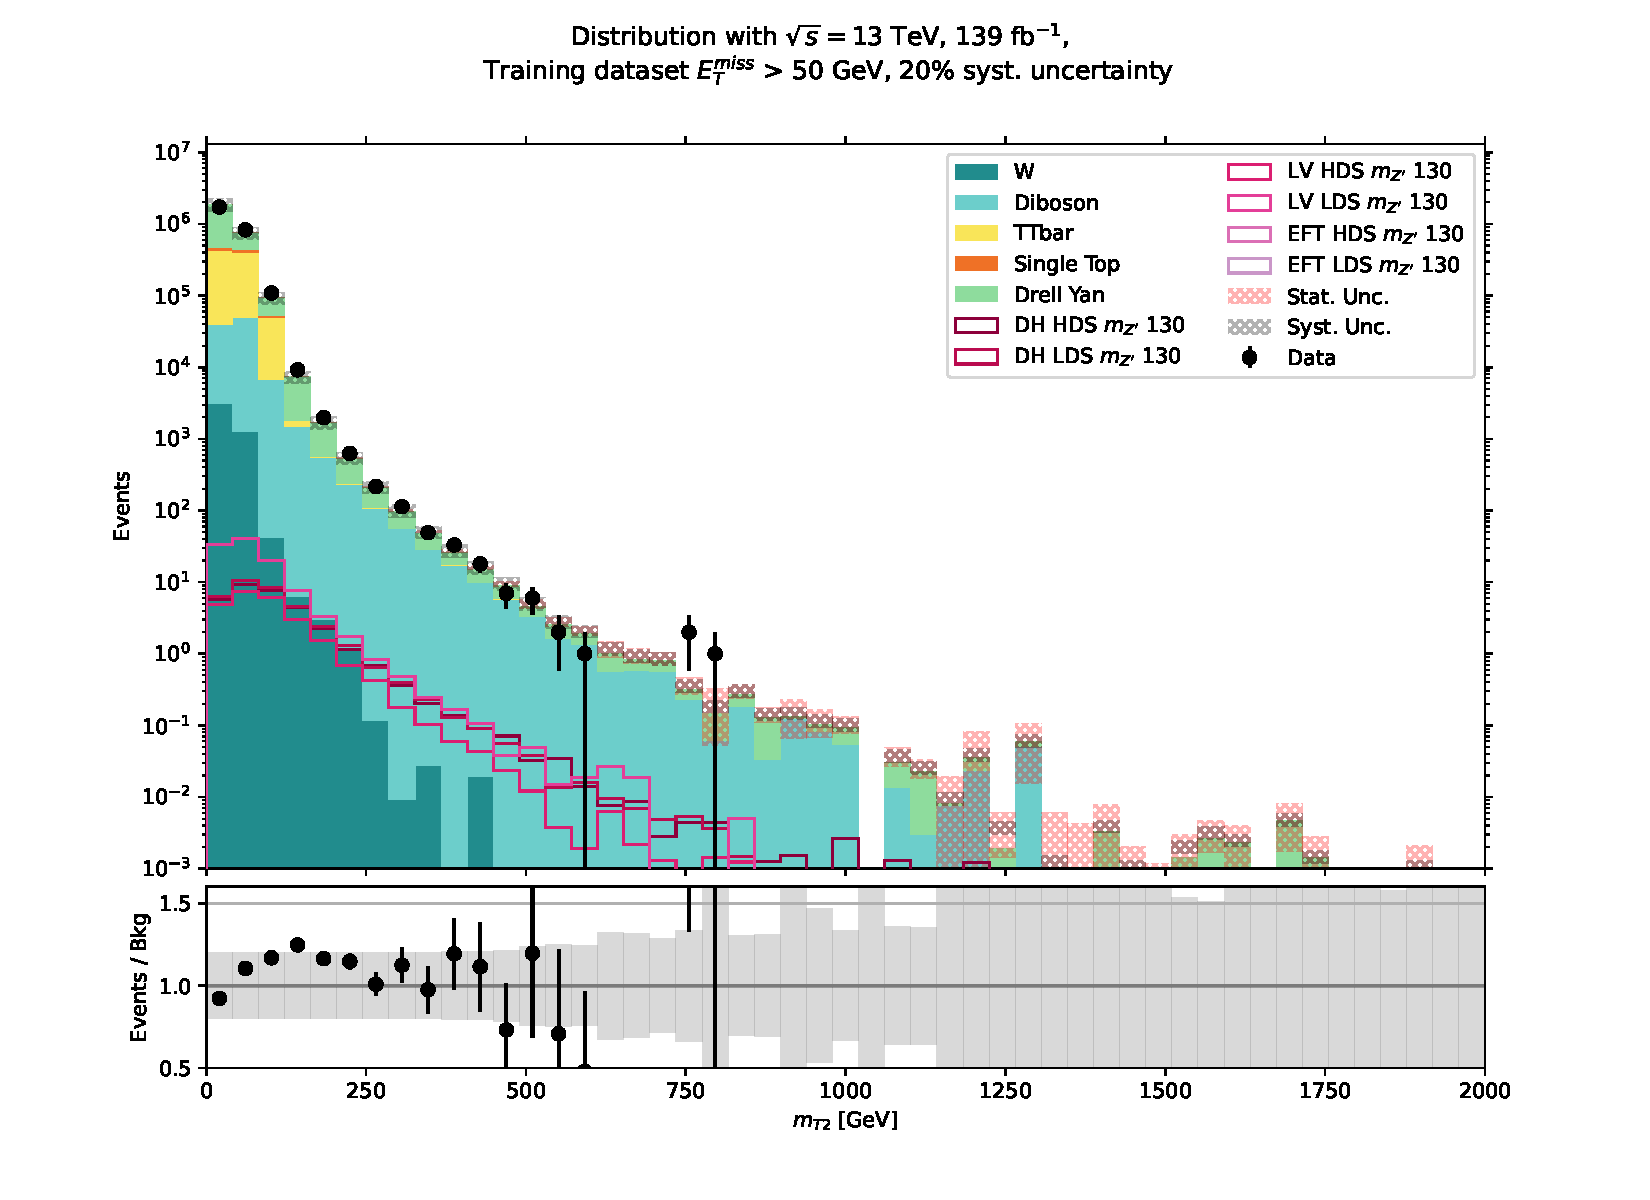
\includegraphics[width=1\textwidth]{mt2_train.pdf}
        \caption{Training distribution}
     \end{subfigure}
     \hfill
     \begin{subfigure}[b]{0.49\textwidth}
        \centering
        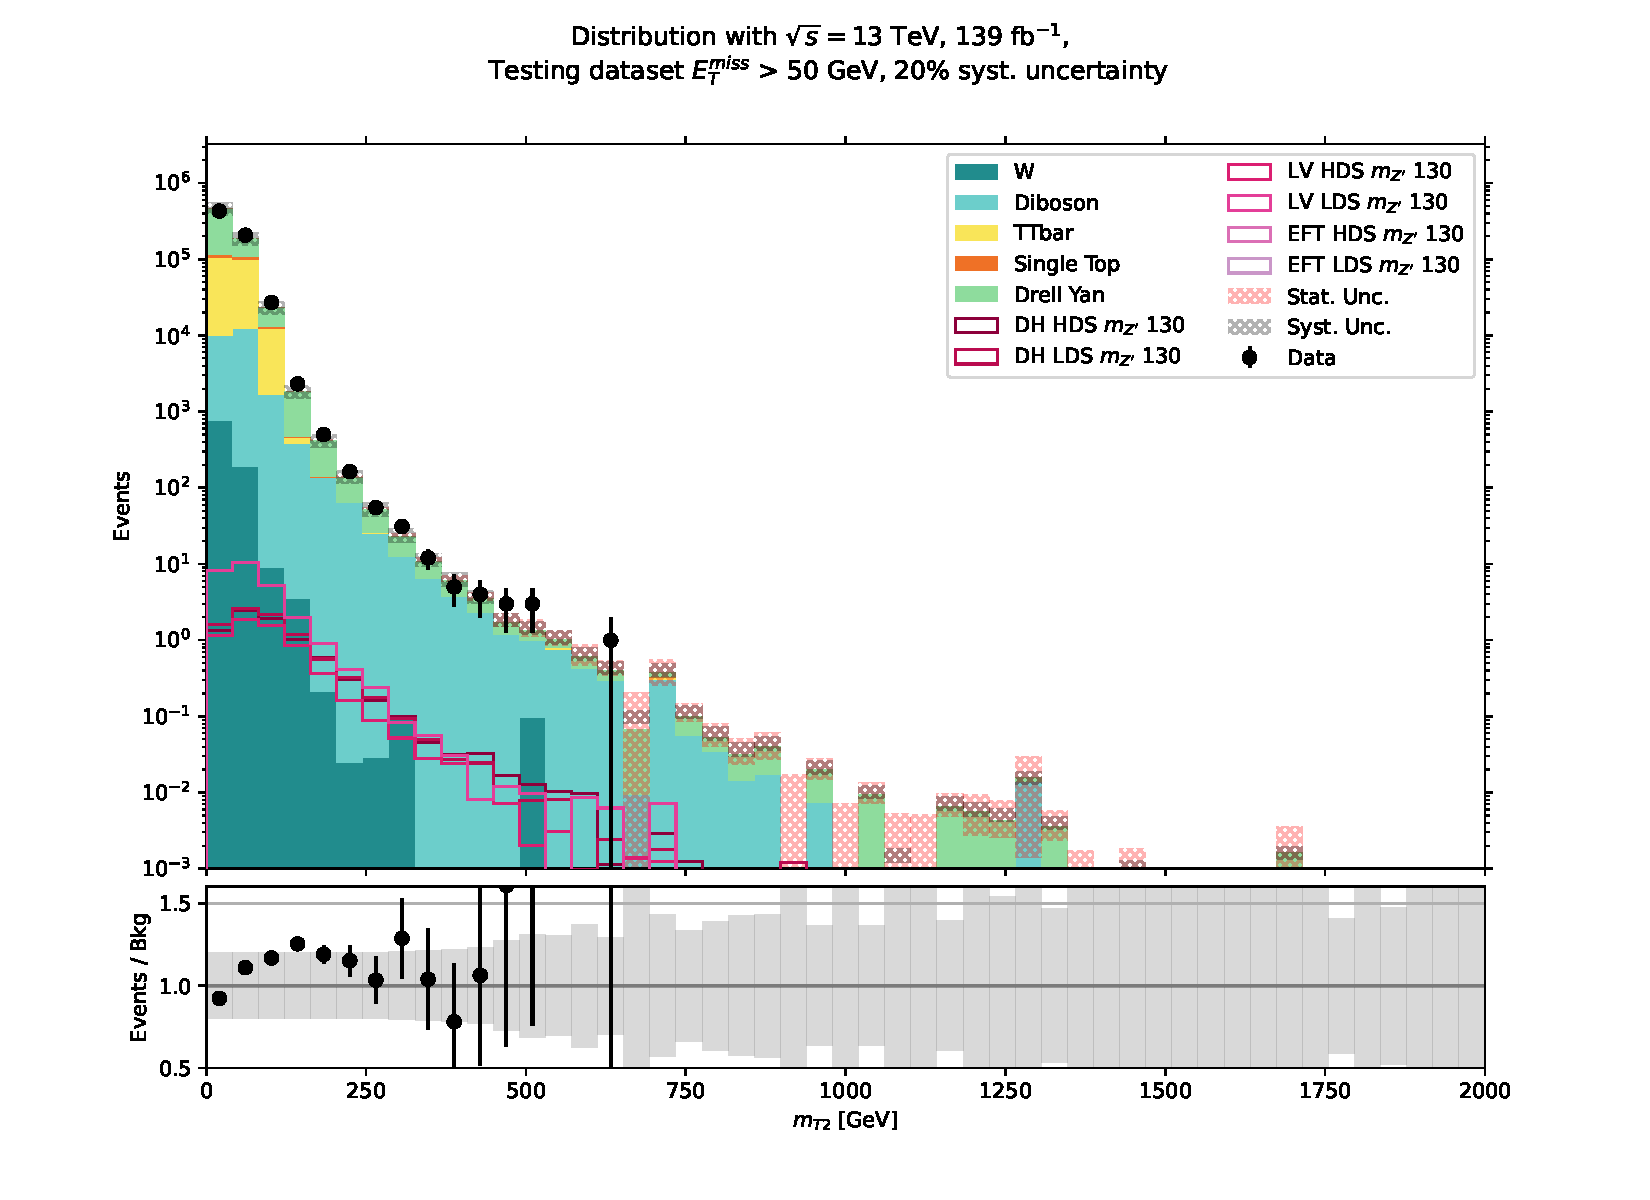
\includegraphics[width=1\textwidth]{mt2_test.pdf}
        \caption{Testing distribution}
     \end{subfigure}
	\caption[Train-test split distribution]{Distribution of the stransverse mass when dividing SM background and DM samples into 80\% training and 20\% testing datasets. The integrated luminosity for each distribution is 80\% and 20\% of 139 $fb^{-1}$ respectively. We also included an estimated 20\% flat systematic uncertainty to the simulated events.}\label{fig:train-test}
\end{figure}
\\In Figure \ref{fig:train-test} we can see that the distribution has not been altered when we split the dataset into 80-20. The data and MC agree reasonably in both datasets, meaning the distributions are split correctly. To see the distribution of every other kinematical variable see the GitHub repo\footnote{Available here: \href{https://github.com/rubenguevara/Master-Thesis/tree/master/Plots/Data_Analysis/train_test_split}{https://github.com/rubenguevara/Master-Thesis/tree/master/Plots/\\Data\_Analysis/train\_test\_split}}.


\clearpage
\section{Neural Network Training}\label{chap:NN_train}
For this thesis we utilize \verb|TensorFlow v. 2.7.1 GPU| for all NNs. After creating the dataset, the first and most important thing is to marinate the \verb|batch_size| whenever we try anything while using the dataset. This is to optimize wrt. to both the size 
of the dataset and the imbalance between signal and background events.\\
\\The highest possible batch size that could be used for this thesis was $2^{22}$,\footnote{It has to be a power of two because of the alignment of virtual processors (VP) onto physical processors (PP) of the GPU. As the number of PP is often a power of 2, using a number of VP different from a power of 2 leads to poor performance.} 
leading to roughly 4 million simulated events per batch. This is the best that a dedicated GPU, \verb|NVIDIA A100-PCIE-40GB|, could handle. The batch size also decreases the more complex the NN becomes, as this requires greater computational power. If we reduce the batch size for any of the tests we will explicitly mention what we changed it to.\\
\\With this out of the way there are still a few challenges to mitigate to optimize our NN. These are described below.

\subsection{Padding of data}\label{sec:padding_NN}
There are two difficulties to overcome when utilizing NNs as compared to BDTs. The hardest to solve, as there is no general solution yet, is the padding of \textit{jagged arrays}. As indicated in Table \ref{tab:variables} with the $^\dagger$, we will record events 
with up to three jets in the final state. However, there are not always three jets in the recorded events that we will be studying, this creates jagged arrays which we can interpret as arrays with missing values. This is an unwanted feature that we need to avoid when 
training NNs.\\
\\To mediate this problem we chose to set the $p_T$ to zero for the missing jets and $m_{jj}$ to zero if there are less than two jets, this is something that is physically reasonable as it does not violate any conservation laws. 
More problematic however is the $\eta$ and $\phi$ when there are no jets. To mediate this we have set the values to -999, which has no physical meaning and is impossible to achieve, this we did so it becomes easier for us to identify the jagged arrays that 
need different interventions.\\
\\As mentioned before, there is no consensus on how the padding should be done, and there are many methods of doing so. The classical data scientist way of solving this problem would be to just take 
the mean of every feature and use that as a variable for every event with missing values. That means replacing every $p_T, m_{jj} = 0$ and $\eta,\phi=-999$ with the mean of every $p_T$, $m_{jj}$, $\eta$ and $\phi$ (excluding the 0's and -999's respectively). 
However, this is not popular among physicists since it breaks conservation laws when we say there are jets present in an event when in reality there are none. Another approach is to use Bayesian statistics or ML to estimate the missing values, 
these options will not be pursued in this thesis due to time constraints, but might be of interest for future projects. Another approach, is setting all the missing values to zero, as this might mean that there is not anything there, 
but this also breaks conservation laws since $\eta,\phi=0$ have physical meaning, this is also highly looked down upon by data scientists since this could affect the weighting when training the network and potentially create a false pattern for the network to follow which would lead to a bias.\\ 
\\The jet $p_T$ and $m_{jj}$ being 0 is a valid form of padding the dataset, as this does not break any fundamental law of physics. However, setting $\phi$ as something outside $[-\pi,\pi]$ does not make much sense 
as this is the angle around the detector. Setting a high value of $\abs{\eta}$ might be possible in principle, but as of today the ATLAS detector has a $\abs{\eta}<4.9$ (see Chapter \ref{sec:ATLAS}) as the pseudorapidity 
states how close to the beam line the objects recorded are. However, having a $p_T$ of a jet equal to zero while still recording the $\eta$ and $\phi$ breaks the laws of physics, so this is a problem that needs to be fixed.\\
\\Another approach is to remove the features with missing values to conserve statistics, albeit make it harder for the network to see any pattern that we might miss, but this is also not a desirable mitigation. 
Instead, we have tried to limit ourselves to the use of number of jets of defined categories that work around the need of padding. These features are just \textit{event features}, meaning that we count the number of jets that fulfill some criteria, 
such as the number of b-jets with $p_T > 20$ GeV, the number of light jets with $p_T>40$ GeV, the number of jets recorded in the central calorimeter ($\abs{\eta} < 2.5$), and the number of 
jets with $p_T>50$ GeV recorded in the forward calorimeter ($\abs{\eta} > 2.5$). The $p_T$ cuts are optimized to allow a good agreement between data and simulations, the distributions can be seen in the GitHub repo. 
The padding variables included in the training are shown in Table \ref{tab:padding_variables}.\\
\begin{table}[!h]
   \centering
   \caption[New features that need no padding]{Table showcasing features that will not need padding.}
   \begin{tabular}{l|r}\midrule\midrule
      Kinematic variable                                                      & Feature name          \\\midrule
      Number of b-jets with $p_T > 20$ GeV                                    & n\_bjetPt20\\
      Number of light-jets with $p_T > 40$ GeV                                & n\_ljetPt40\\
      Number of jets recorded in Central calorimeter                          &n\_jetsetaCentral\\
      Number of jets recorded in Forward calorimeter with $p_T > 50$ GeV      & n\_jetsetaForward50\\\midrule\midrule
   \end{tabular}
   \label{tab:padding_variables}
\end{table}
\\When training our NN with these new variables instead of dropping features with missing variables we hope that the NN learns more physics by hopefully recognizing patterns between all high level features. Having addressed the challenge of jagged arrays, we will continue to 
address the second step to prepare the dataset for the NN, the normalization procedure. 

\subsection{Normalization of data}\label{sec:normie_NN}
Since neural networks send a lot of data into multiple neurons and multiple layers using activation functions and carrying weights and biases that change 
for every back propagation iteration, it is important to make sure that a neuron output does not vanish when moving around the network. Meaning that a neuron output becomes negligible compared to others when navigating the loss-phase space.
A fast way for a neuron output's to vanish is to not normalize the data and send it through the network as it is available. The reason it might vanish, is because we send in numbers which vary significantly from each other, i.e. the $p_{T}$ might be as high as thousands GeV, while 
$E_T^{miss}/\sigma$ might be as low as 0.1. What might happen when sending such different numbers is that the network might think "obviously the high number is more important than the low number" thus making the activation function worse for the feature, even though 
this feature is of high importance when looking at MET final states. A way to fix this problem is to normalize all features. There are many ways to do this, one could do \textit{min max scaling} which normalizes every feature from $[0,1]$, completely solving the problem above. 
Mathematically speaking this is done by
\begin{equation}\label{eq:minmax}
   X_{norm} = \frac{X - X_{min}}{X_{max}-X_{min}}
\end{equation}
Where $X$ is the array containing all events for a given feature, while $X_{min}$ and $X_{max}$ are the lowest and highest values in the said array. Another way to normalize the data is to make the mean of every feature such that the mean of all the features is distributed according 
to a standard normal distribution (mean 0 and std. 1), this is called \textit{Z-score normalization}
\begin{equation}\label{eq:Z-score}
   X_{norm} = \frac{X - \bar{X}}{\sqrt{\sigma_X^2}}
\end{equation}
where $\bar{X}$ is the mean of said array and $\sigma_X^2$ is the variance. One could also use pre-built functions in \verb|TensorFlow| that provide a normalization, such as \verb|Batch_normalization| of the data entering the network per batch. This is usually used 
in Convolutional NN's as it improves computational speed. Another one, \verb|Normalize|, provides the same as Eq. (\ref{eq:Z-score}) for the whole training set going in. This is however computationally heavy to use. The \verb|Layer_normalization|, which normalizes the activations 
of the previous layer in a batch \textit{independently}, rather than \textit{across} a batch like \verb|Batch_Normalization|. Both \verb|Batch_Normalization| and \verb|Layer_Normalization| use an optimized version of the Z-score when normalizing the data, meaning that all the features 
take are normalized following a standard normal distribution.\\
\\There is a big difference when normalizing data ourselves or using \verb|TensorFlow|. \verb|TensorFlow| remembers how the data was normalized when training such that the test data will be normalized the same way, making testing easier. While if we use Eq. (\ref{eq:minmax}) or 
Eq. (\ref{eq:Z-score}) ourselves, we have to make sure that we use the same values for $X_{max}, X_{min}, \bar{X}$ or $\sigma_X^2$ when normalizing the test data. 



\subsection{Balancing of signal and background}\label{sec:balance_NN}
The biggest challenge to overcome in this thesis is what we should use as sample weights (see Section \ref{sec:sample_weight}). If we were to not use any form of sample weights to mitigate the imbalance in our data set it could potentially lead to \textit{majority class classification} where the 
networks could get "lazy" and guess that everything is background. \\
\\To combat the majority class classification, we will as mentioned make use of the sample weights. We will study three cases
\begin{enumerate}
   \item Unweighted training, meaning that we will be setting the sample weight to one
   \item Weighted training, meaning that we will be setting the sample weight to the weights used to re-weight MC events to the expected events as explained in Chapter \ref{sec:wgts}
   \item Balanced training, we will weigh the background and signal samples in an attempt to balance the number of events available in each of the two categories,
\end{enumerate}
where the latter would in terms of weights mimic a 50-50 distribution of signal and background. 

\subsection{Re-weighting MC to expected events}\label{sec:sample_wgts_NN}
Even if the weighting method previously described might help the NN give us better results, we also want to include the weights used to re-weight MC events to expected events. This is desirable in the sense that we want to show our ML networks the true kinematical distributions of each feature.
As the re-weighting weights are generated with simulation corrections as well as luminosity and cross-section in mind, it is heavily desirable to also apply these corrections when training our networks, such that it can correctly make predictions in the test dataset regardless of their weight. This is particularly 
crucial when using real data on our predictions, as these have no weights.\\
\\Ideally one would take into account both the data imbalance between the signal and background as well as the re-weighting weights when training a network. To do this using \verb|TensorFlow| we could make use of two parameters when training the network: \verb|class_weight| and \verb|sample_weight|. The
\verb|class_weight| works as a dictionary that weighs events differently, based on a dictionary key, for our purposes this key would be whether the event is a signal or background event. 
The \verb|sample_weight| takes in individual weights for every single event that goes into the network, meaning that it is crucial that we know that the desired weight matches the desired event. Ideally we would use both weighting methods, \verb|class_weight| to balance the signal to 
background ratio and \verb|sample_weight| with the re-weighting weights that include the cross-section. However, there is a bug in \verb|TensorFlow| (up to version \verb|GPU 2.7.1|) that prevents the program to run when using both parameters. This is not a big problem though, as when looking at the source code \cite{Keras_source_code} 
one can see that what \verb|TensorFlow| does with both weights is multiply them together. This means that to mitigate this problem we will use element-wise multiplication between the re-weighting weights array and the balancing weights array to create a new array that will be used as \verb|sample_weights|. \\
\\For this thesis we tried testing four different methods to make the sample weights. For the re-weighting array, all background events will be re-weighted to expected events using the weights from Section \ref{sec:wgts} while the signal events will have a value of one.  %\footnote{The reason we do not re-weight the signal events is both because we do not actually know what the cross-section is, and because the cross-section is so low compared to the SM that it would punish the ML algorithm}, 
The balancing array was made by expanding the balancing ratio from Section \ref{sec:balance_NN} to be
\begin{enumerate}
   \item $\frac{N_{sig,MC}}{N_{bkg,MC}}$ where we weigh down all background events wrt. the ratio of total simulated signal events over the total simulated background events
   \item $\frac{N_{bkg,MC}}{N_{sig,MC}}$ where we weigh up all signal events wrt. the ratio of total simulated background events over the total simulated signal events
   \item $\frac{N_{sig,MC}}{N_{bkg,exp}}$ where we weigh down all background events wrt. the ratio of total simulated signal events over the total expected background events at 139 fb$^{-1}$
   \item $\frac{N_{bkg,exp}}{N_{sig,MC}}$ where we weigh up all signal events wrt. the ratio of expected background events at 139 fb$^{-1}$ over the total simulated signal events, 
\end{enumerate}
and one if we do not weight the event. Note that we are not re-weighting the signal events to expected signal events when training because this would in principle remove all expected events (due small cross-sections) from the NN as there are so few events (see Table \ref{tab:dataset}). 
Taken all of these factors into account what remains is to choose a network architecture and which hyperparameters to use to best fit our task.


\clearpage
\subsection{Architecture and hyperparameter tuning}\label{sec:NNgriddy}
The architecture of the NN utilized in this project is of the form shown in Figure \ref{fig:FFN}, where a NN with an arbitrary number of layers is shown, each of the hidden layers use the ReLu (Eq. (\ref{eq:ReLU})) activation function, and where the output is in the form of a single neuron using the sigmoid activation function (Eq. (\ref{eq:sig})). 
An algorithm showing one possible way to create this NN can be seen in Appendix \ref{alg:nn}. To get the best performance on our NN, we need to find which hyperparameters help the network reach the highest significance. To do this, we need to do a grid search. 
For our neural network we will mainly focus on four hyperparameters explained in section \ref{sec:theory_nn}:
\begin{itemize}
   \item The learning rate $\eta$
   \item The L2-regressor variable $\lambda$
   \item The number of neurons on each hidden layer \verb|n_neuron|
   \item The number of layers \verb|n_layers|, excluding the output. Meaning that \verb|n_layers| = 1 means no hidden layer
\end{itemize}
The metrics that will be used to estimate the best hyperparameters are Area Under the curve (AUC), binary accuracy and most importantly the expected significance\footnote{See Chapter \ref{sec:tools} for explanation of metrics.}.
The expected significance for this section has been calculated using the low statistics formula Eq. (\ref{eq:exp_sig}) without uncertainties. The expected significance will be calculated by making a lower cut of 0.85 on the network prediction score, as explained in Chapter \ref{sec:siggy}. 
For some models where the expected events are too low, the expected significance will be 0 or \verb|NaN|. If this happens we will use the AUC on the testing set as a metric to find the best hyperparameters. 
This procedure will be performed for every single network we will explore. The results of the best method used to optimize NNs is showcased in Section \ref{sec:opt_res}, and a more in depth showcase of the methods can be seen in Appendix \ref{chap:network_opt}. In the next section we will discuss the optimization of BDTs. 
\clearpage


\section{Boosted Decision Tree Training}
When working with BDTs there are not as many challenges to overcome as with NNs. For example the padding and normalization of data can be completely avoided, making the whole procedure a lot easier when one uses challenging dataset as we do in high energy physics.
The weights are still an obstacle that we need to overcome when using BDTs. This will be discussed in Section \ref{sec:bdt_wgts}.\\
\\For this project we will, as mentioned utilize, the eXtreme Gradient Boosting, or \verb|XGBoost| for short, package \cite{XGBoost} made for the Higgs ML Challenge \cite{HiggsChallenge} whenever we mention BDTs.
This project utilized version \verb|1.5.0| without GPU adaptability. \verb|XGBoost| also helps to avoid padding as it is integrated with a \verb|missing_variable| variable where we can simply write the number of the variable that is missing. For the dataset in this project this implies setting the \verb|missing_variable| value to -999, 

\subsection{Sample weights}\label{sec:bdt_wgts}
For \verb|XGBoost| there is a different problem when it comes to weights. XGBoost has a variable called \verb|scale_pos_weight| where we can help the network deal with imbalanced data, such as the one we have. 
Meaning that the whole problem of combining the re-weighting weights with the balancing weights from Chapter \ref{sec:sample_wgts_NN} completely disappears. Albeit there is a caveat, \verb|XGBoost| does not have the possibility to include negative weights, which the datasets explored in this work have. The reason \verb|XGBoost| 
does not include negative weights, is because when calculating the number of events in a leaf node, which is made by taking the sum of sample weights, we cannot have a negative value \cite{neg_wgt_xbg1, neg_wgt_xbg2}.
As for the MC generators, Sherpa \cite{Sherpa} takes into account higher order diagrams and needs to add negative weights to "counter" the over counting of diagrams \cite{Negative_Weights_article}, which are important to correctly scale the simulated events to real data.\\
\\A method to mitigate this problem is to use the absolute value of the weights when training. This is however not generally accepted as a solution, and some even say it should be avoided. There are other options however, one of these options is to not include events with negative weights in the training set. 
This is an okay thing to do, as we can imagine that if we were to only include events with positive weights in the training, it might be the same as putting the negative weights in the "testing dataset" (Chapter \ref{sec:train_test}). 
However, both methods are equally problematic if the positive and negative weights distributions are not equal for all the features.\\
\\Another method that has been used in a published ATLAS article \cite{Abbott:2714377} is to normalize the weights when using the absolute value with respect to the sum of weights over the sum of absolute weights. The reason behind this is that the sum of weights is obviously not the same when we take the absolute value. 
Mathematically speaking, if we have an array of weights $W$, we can update this like
\begin{equation}\label{eq:ATLAS_wgt}
   W \rightarrow \abs{W}\frac{\sum_i W_i}{\sum_i\abs{W_i}}
\end{equation}
such that the weights are at least on the same scale. 

\subsection{Architecture and hyperparameter tuning}\label{sec:BDTGriddy}
Making a BDT for our purposes is fairly easy as well using XGBoost. One way to do it is using the algorithm shown in Algorithm \ref{alg:xgb}. 
To get the best performance on our BDT we have to do a grid search here as well. The trainable hyperparameters here are different from NN's, with XGBoost we will focus on the following hyperparameters
\begin{itemize}
   \item Tree depth: how many times we split the data
   \item Number of estimators: how many trees we use to do the gradient boosting
   \item The learning rate $\eta$
   \item L2-regressor $\lambda$, to stop overtraining
\end{itemize}
The same procedure for hyperparameter optimizations as described for NNs in Section \ref{sec:NNgriddy} will be used for BDTs as well. The results of the best method used to optimize BDTs is showcased in the next section, a more in depth showcase of the methods can be seen in Appendix \ref{chap:network_opt}. 

\newpage
\section{Results of optimization methods}\label{sec:opt_res}
We tested the normalization, balancing of signal and background, re-weighting of events using NNs, as well as the use of sample weights with BDTs. In this section of the thesis we show the main result of the network optimization procedure, the full results are detailed in Appendix \ref{chap:network_opt}. We observed that for the NNs using \verb|Batch_normalization| as the normalization method yielded better results, 
we also saw that the NN was better at sorting signal from background using ADAM as the optimizer rather than using SGD. 
Concerning the sample weights, the method that yielded the best results was the one that re-weighted every simulated background event into the expected events with a luminosity of 139 fb$^{-1}$, and balanced the dataset by weighing up all signal events by the ratio of expected number of background events over simulated signal events, $\frac{N_{bkg,exp}}{N_{sig,MC}}$. We also observed that the new padding method, 
which counted the number of (light)b-jets with $p_T>(40)20$ GeV, the number of jets in the central calorimeter, and the number of jets with $p_T>40$ GeV in the forwards calorimeter, performed better than the other method of removing jet features with missing variables. \\
\\For the BDT we observed that while conducting a grid search for the optimal hyperparameters, we never hit a plateau where the scores seemed to flatten out when increasing the tree depth. However, we decided to take the conservative approach of having a tree depth of maximum 6. The sample weights we decided to use further with BDTs were the ones 
that only looked at the positive weights of the dataset, instead of using the scaled up absolute value of the weights. To balance the signal and background events in the dataset we weighed down the background events with the ratio of total simulated signal events over the total expected background events at 139 fb$^{-1}$.\\
\\The best results from the BDT and NN trained using the model dependent approach on the Dark Higgs Heavy Dark Sector model are compared in Figure \ref{fig:BDT_vs_NN}.
\newpage
\begin{figure}[!ht]
	\centering
   \graphicspath{{../../../Plots/XGBoost/Weighting_methods/}}
   \begin{subfigure}[b]{0.49\textwidth}
      \centering
      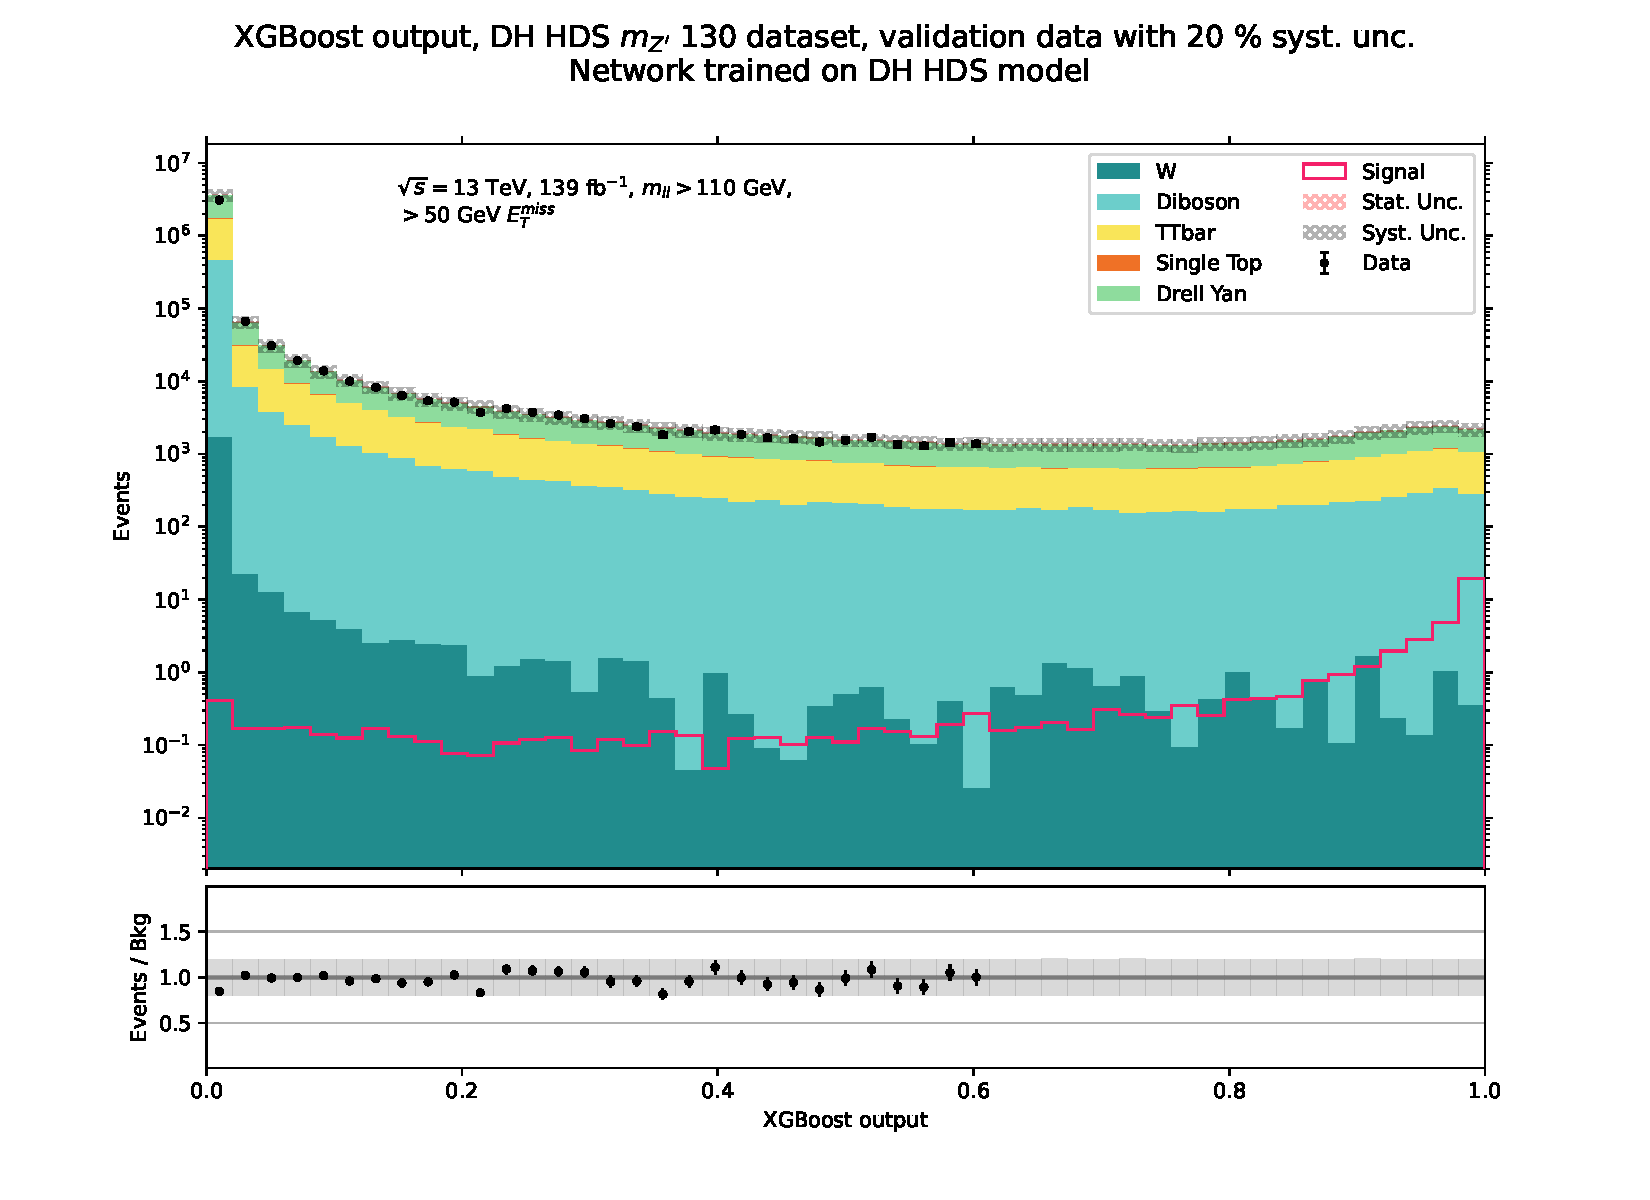
\includegraphics[width=1\textwidth]{Pos_wgt/VAL.pdf}
      \caption{BDT result}
   \end{subfigure}
   \graphicspath{{../../../Plots/NeuralNetwork/Padding/}}
   \begin{subfigure}[b]{0.49\textwidth}
      \centering
      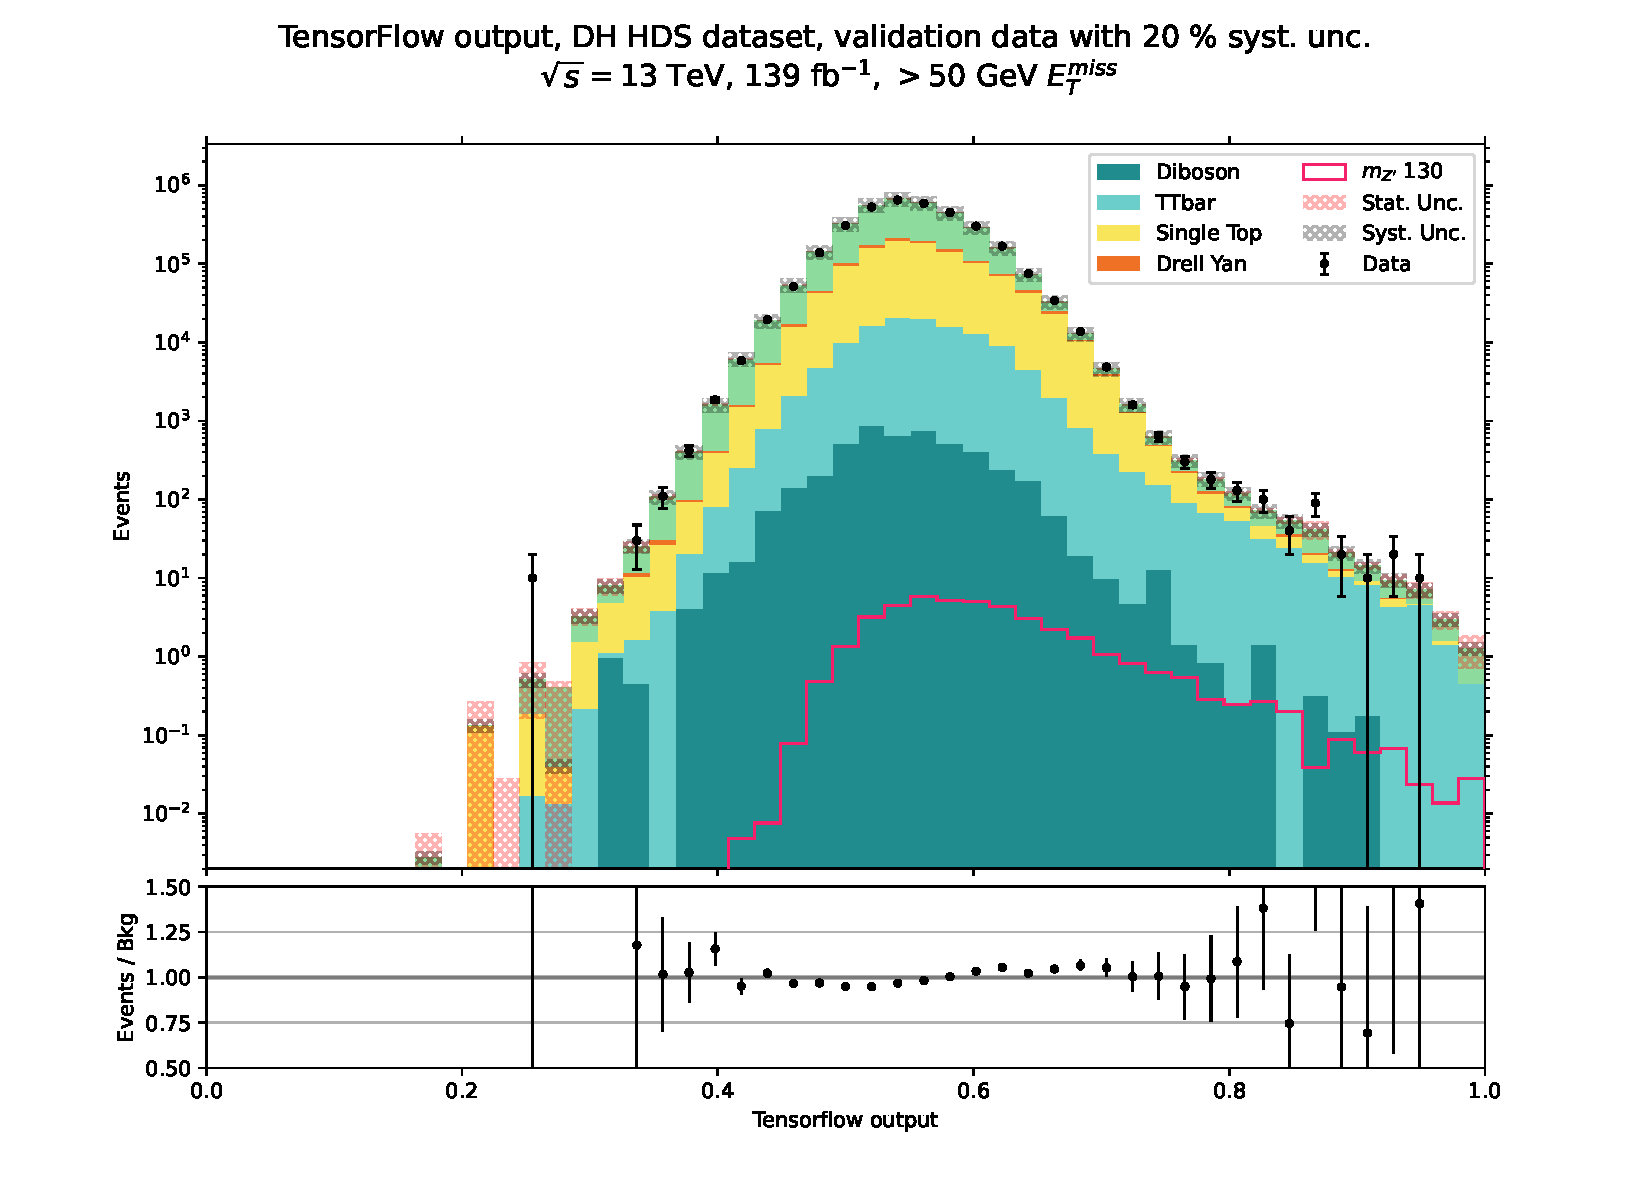
\includegraphics[width=1\textwidth]{New_pad/VAL.pdf}
      \caption{NN result}
   \end{subfigure}
   \graphicspath{{../../../Plots/XGBoost/Weighting_methods/}}
   \begin{subfigure}[b]{0.49\textwidth}
      \centering
      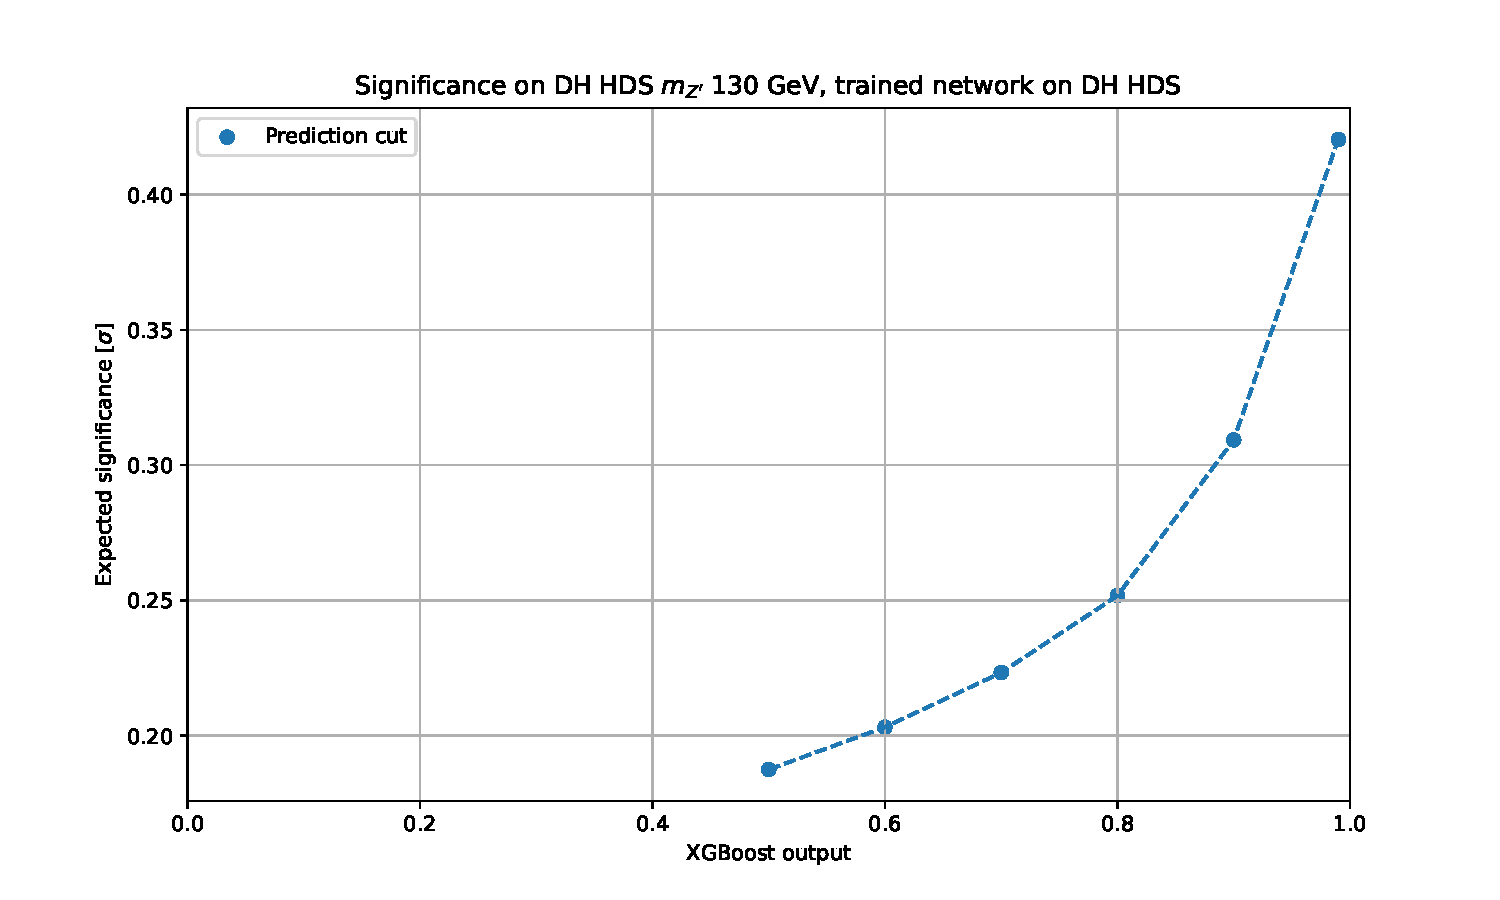
\includegraphics[width=1\textwidth]{Pos_wgt/EXP_SIG.pdf}
      \caption{Significance of (a)}
   \end{subfigure}
   \graphicspath{{../../../Plots/NeuralNetwork/Padding/}}
   \begin{subfigure}[b]{0.49\textwidth}
      \centering
      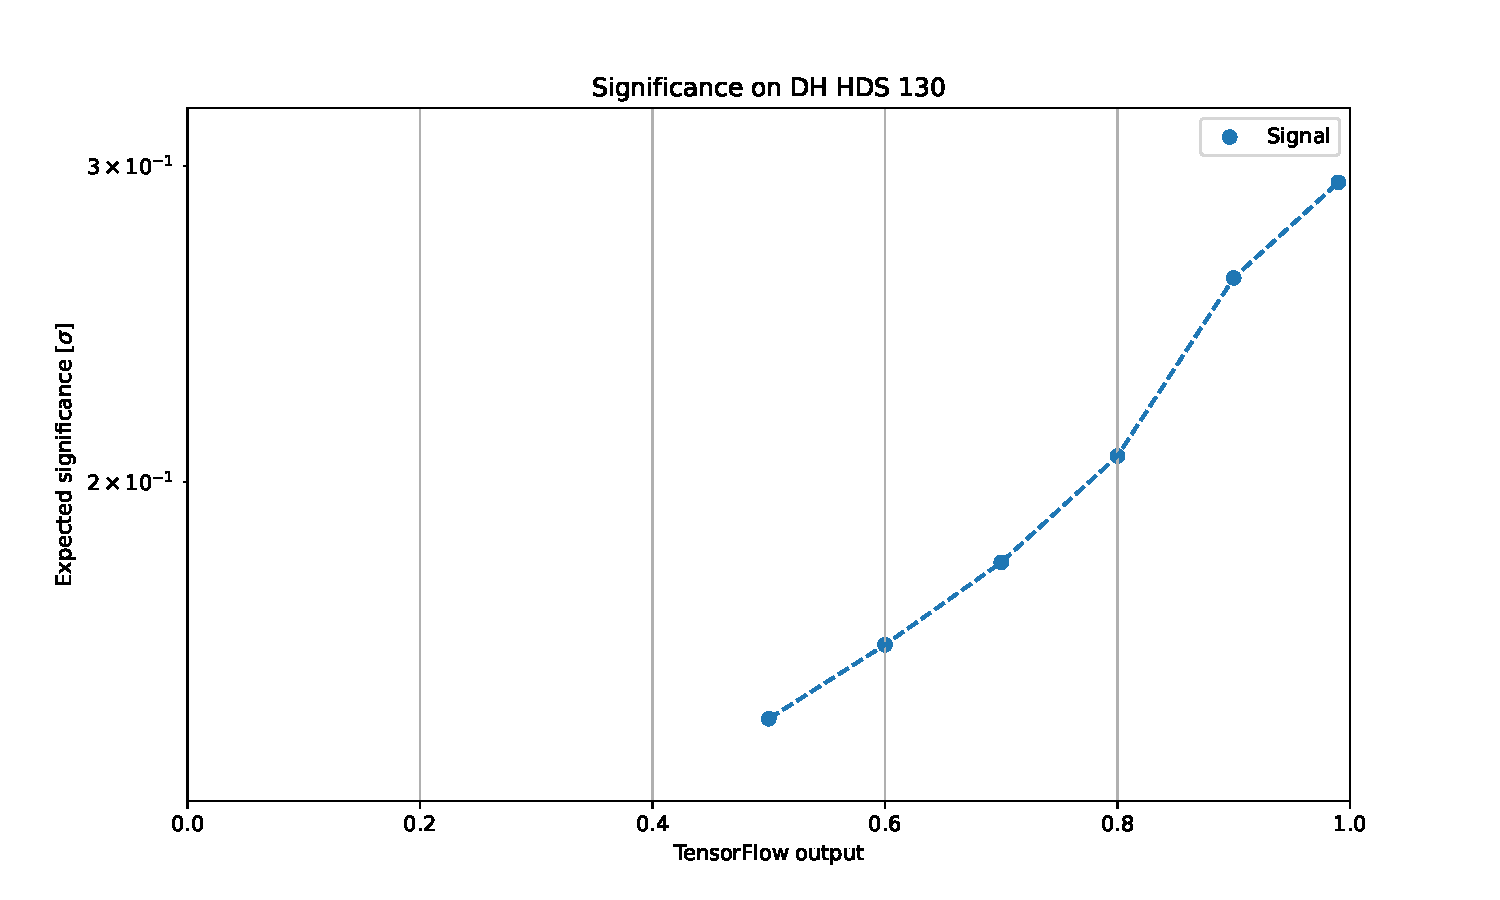
\includegraphics[width=1\textwidth]{New_pad/EXP_SIG.pdf}
      \caption{Significance of (b)}
   \end{subfigure}
   \caption[Comparison of BDT and NN]{Comparison of BDT and NN. Both networks were tested on the DH HDM dataset using the model dependent approach. The output on the x-axis on all plots above reflects the score of the ML output ranging from 0-1, where 1 means that the ML network classifies an event as signal and 0 means background. In plot (a) and (b) we can see the distribution of events given the output. In plot (c) and (d) we see the expected significance as a function of the low cut on the output. }\label{fig:BDT_vs_NN}
\end{figure}
\noindent Figure \ref{fig:BDT_vs_NN} showcases the ML distribution score from 0-1\footnote{Where 0 means background and 1 means signal} for every event using both algorithms (upper plots), and the expected significance from the distribution plots as a function of the lower cut on the output. From the results we can see that the BDTs perform better than NNs as the expected significance on the last bin is higher by $\approx0.13\sigma$. As using BDTs is easier than NNs, 
as well as BDTs having greater interpretability, we will for the remainder of the thesis opt to only use BDTs as our main ML algorithm. We have now explored the methods that will be used for this search, and all the challenges that need to be mitigated. The next part of this thesis will present 
the results of both the model dependent and independent approach for every model. 




\end{document}